\documentclass[parskip=half]{scrartcl}
\usepackage[utf8]{inputenc}
\usepackage{amsmath}
\usepackage{amssymb}
\usepackage{graphicx}
\usepackage{authblk}
\PassOptionsToPackage{hyphens}{url}
\usepackage[hidelinks]{hyperref}
\usepackage{listings}
\lstset{basicstyle=\ttfamily}
\usepackage{enumitem}
\setlist[enumerate]{itemsep=0mm}
\setlist[itemize]{itemsep=0mm}

% Cross referencing external documents.
\usepackage{xr}
% Command for registering file dependencies with latexmk.
\makeatletter
\newcommand*{\addFileDependency}[1]{% argument=file name and extension
  \typeout{(#1)}
  \@addtofilelist{#1}
  \IfFileExists{#1}{}{\typeout{No file #1.}}
}
\makeatother

\externaldocument[s-]{supplement}
\addFileDependency{supplement.tex}
\addFileDependency{supplement.aux}

\usepackage[maxbibnames=999,backend=bibtex]{biblatex}
\addbibresource{literature.bib}

\newcommand{\sharedfirst}{$\dagger$}
\newcommand{\sharedfirsttext}[1]{\affil[\sharedfirst]{#1}}
\newcommand{\corresponding}{*}
\newcommand{\correspondingtext}[1]{\affil[\corresponding]{#1}}
\newcommand{\image}[1]{\centering\includegraphics[width=\textwidth]{#1}}
\let\plainurl\url
\renewcommand{\url}[1]{\protect\plainurl{#1}}

\begin{document}

\author[1,2]{Felix Mölder}
\author[6]{Kim Philip Jablonski}
\author[4]{Michael Hall}
\author[4]{Brice Letcher}
\author[5]{Vanessa Sochat}
\author[3]{Soo Lee}
\author[8]{Sven~O.~Twardziok}
\author[9]{Alexander Kanitz}
\author[14]{Andreas Wilm}
\author[1,13]{Jan Forster}
\author[10,8]{Manuel Holtgrewe}
\author[11]{Chris Tomkins-Tinch}
\author[12]{Sven Nahnsen}
\author[1,7,\corresponding]{Johannes Köster}

\affil[1]{Algorithms for reproducible bioinformatics, Genome Informatics, Institute of Human Genetics, University Hospital Essen, University of Duisburg-Essen, Essen, Germany}
\affil[2]{Institute of Pathology, University Hospital Essen, University of Duisburg-Essen, Essen, Germany}
\affil[3]{Biomedical Informatics, Harvard Medical School, Harvard University, Boston, USA}
\affil[4]{TODO EMBL-EBI}
\affil[5]{TODO Stanford Computing, Stanford University}
\affil[6]{TODO ETH Zürich}
\affil[7]{Medical Oncology, Harvard Medical School, Harvard University, Boston, USA}
\affil[8]{Charité - Universitätsmedizin Berlin, corporate member of Freie Universität Berlin, Humboldt-Universität zu Berlin, and Berlin Institute of Health (BIH), Center for Digital Health, Berlin, Germany}
\affil[9]{Biozentrum, University of Basel, Switzerland \& SIB Swiss Institute of Bioinformatics / ELIXIR Switzerland, Lausanne, Switzerland}
\affil[10]{CUBI – Core Unit Bioinformatics, Berlin Institute of Health, Berlin, Germany}
\affil[11]{TODO}
\affil[12]{TODO}
\affil[13]{TODO}
\affil[14]{TODO}
\sharedfirsttext{Shared first author}
\correspondingtext{To whom correspondence should be addressed}

\title{Sustainable data analysis with Snakemake}
\maketitle

\begin{abstract}
	Data analysis often entails a multitude of heterogeneous steps, from the application of various command line tools to the usage of scripting languages like R or Python for the generation of plots and tables.
	It is widely recognized that such processes have to be conducted in a reproducible way.
	Reproducibility enables to verify the technical validity of a data analysis and to regenerate results on the original or even new data.
	However, reproducibility alone is by no means sufficient to deliver an analysis that is of lasting impact (i.e. sustainable) for the field, or even just the own research group.
	We postulate that it is equally important to ensure adaptability and transparency.
	The former describes the ability to modify the analysis to answer for example extended or slightly different research questions.
	The latter describes the ability to understand the analysis, in order to judge whether it is not only technically, but methodologically valid.

	Here, we analyze the properties needed for a data analysis to become reproducible, adaptable and transparent, and show how the popular workflow management system Snakemake can be used to fulfill all these needs.
\end{abstract}

Performing data analysis has become ubiquitous across scientific disciplines.
Along with that, securing \emph{in silico} reproducibility has been identified as a major challenge~\parencite{Mesirov2010,Baker2016,Munaf__2017}.
In consequence, recent years have seen a wide adoption of scientific workflow management systems by the community and countless workflow management systems have been published (see~\url{https://github.com/pditommaso/awesome-pipeline}).
These can be partitioned into five niches, for which we will highlight the major representatives below.

First, workflow management systems like Galaxy~\parencite{Afgan2018} offer a graphical user interface for composition and execution of workflows.
The obvious advantage is the shallow learning curve, making such systems accessible for everybody, without the need for programming skills.

Second, with systems like Anduril~\parencite{Cervera2019}, Balsam~\parencite{papka2018}, Hyperloom~\parencite{cima2018hyperloom}, Jug~\parencite{Coelho_2017}, Pwrake~\parencite{Tanaka_2010}, Ruffus~\parencite{Goodstadt2010}, SciPipe~\parencite{Lampa2019}, SCOOP \parencite{SCOOP_XSEDE2014}, and COMPSs~\parencite{Lordan_2013} workflows are specified using~ a set of classes and functions for generic programming languages like Python, Scala and others.
Such systems have the advantage that they can be used without a graphical interface (e.g. in a server environment), and that workflows can be straighforwardly managed with version control systems like Git (\url{https://git-scm.com}).~ 

Third, with systems like Nextflow~\parencite{Di_Tommaso_2017}, Snakemake~\parencite{Köster2012}, BioQueue~\parencite{Yao2017}, Bpipe~\parencite{Sadedin2012}, ClusterFlow~\parencite{Ewels2016}, Cylc~\parencite{J_Oliver_2018},~and BigDataScript~\parencite{Cingolani_2014}, workflows are specified using a domain specific language (DSL).
Here, the advantages of the second niche are shared, while adding the additional benefit of improved readability since the DSL provides statements and declarations that specifically model central components of workflow management, thereby obviating superfluous operators or boilerplate code.
In case of Nextflow and Snakemake, where the DSL is implemented as an extension to a generic programming language (Groovy and Python), even access to the full power of the underlying programming language is maintained (e.g. for implementing conditional execution and handling configuration).

Fourth, with systems like Popper~\parencite{Jimenez_2017}, workflow specification happens in a purely declarative way, via configuration file formats like YAML.
Here, most of the benefits of the third niche are shared.
In addition, workflow specification can be particularly readable for non developers.
This comes however with the downside of being more restricted since the facilities of imperative or functional programming are not available.

Fifth, there are system-independent workflow specification languages like CWL~\parencite{cwl} and WDL~\parencite{voss_full-stack_2017}.
These define a (declarative) syntax for specifying workflows, which can be parsed and executed by arbitrary executors, e.g. Cromwell (\url{https://cromwell.readthedocs.io}), Toil~\parencite{Vivian_2017}, and Tibanna~\parencite{Lee_2019}.
Here, a main advantage is that the same workflow definition can be executed on various specialized execution backends, thereby promising scalability to virtually any computing platform.

Today, several of the above mentioned approaches support full in silico reproducibility of data analyses (e.g. Galaxy, Nextflow, Snakemake, WDL, CWL), by allowing the definition and automatic scalable execution of each involved step, together with the ability to define and automatically deploy the software stack needed for each step (e.g. via the Conda package manager,~\url{https://docs.conda.io}, or Docker containers~\url{https://www.docker.com}).

Reproducibility is important to generate trust in scientific results.
However, we postulate that a data analysis is of lasting value (and thus sustainable) for the authors and the scientific field only if a hierarchy of additional interdependent properties is ensured (see Fig.~\ref{fig:sustainability}).

\begin{figure}
	\image{sustainability-in-wms.pdf}
	\caption{
		Hierarchy of aspects to consider for sustainable data analysis.
		By supporting the top layer, a workflow management system can promote the center layer, and thereby help to obtain true sustainability.
	}\label{fig:sustainability}
\end{figure}

By being \emph{automated}, \emph{scalable} to various computational platforms and levels of parallelism, and \emph{portable}, in the sense that it is able to be automatically deployed with all required software in exactly the needed versions, a data analysis gains full in silico \emph{reproducibility.
}

While being able to reproduce results is a major achievement, \emph{transparency} is equally important: the validity of results can only be fully assessed if~the parameters, software and custom code of each analysis step is fully accessible.
On the level of the code, a data analysis therefore has to be \emph{readable} and well \emph{documented}.
On the level of the results it has to be possible to \emph{trace} parameters, software stack and code through all involved steps.

Finally, valid results yielded from a reproducible data analysis become even more beneficial for the scientific community once the analysis can be reused for other projects.
In practice, this will almost never be a plain reuse, and instead requires~\emph{adaptability} to new circumstances, e.g. being able to extend the analysis, replace or modify steps and adjust parameter choices.
Such adaptability can only be achieved if the data analysis can easily be executed at a different computational environment (e.g. a different institute), thus it has to be \emph{scalable} and \emph{portable} again.
In addition, it is crucial that the analysis code is as \emph{readable} as possible such that it can be easily modified.

In this work, we show how sustainability in terms of these aspects is supported by Snakemake.
Since its original publication in 2012, Snakemake has gained a wide adoption, culminating in, on average, nowadays more than three new citations per week, and over 600 citations in total (Fig.~\ref{fig:citations}), making it one of the most widely used workflow management systems in science.

\begin{figure}
	\image{citations.pdf}
	\caption{
		Citations of the original Snakemake article, (a) by year, (b) by scientific discipline of the citing article.
		Data source:~\url{https://badge.dimensions.ai/details/id/pub.1018944052}, 2020/05/20.
	}
	\label{fig:citations}
\end{figure}

We first present several central and novel contributions to the field implemented in Snakemake.
Second, we show how Snakemake comprehensively covers data analysis needs by introducing generic workflow design patterns that can serve as blueprints for composing any kind of analysis.

\section{Results}

In the following, we describe how sustainability is achieved with Snakemake by following the central goals outlined above.

\subsection{Automation}\label{sec:automation}

The key idea of Snakemake is that workflows are specified by decomposing them into steps, which are represented as~\emph{rules~}(Fig.~\ref{fig:example}).
Each rule describes how to obtain a set of output files from a set of input files.
This can happen via a shell command, a block of Python code, an external script (Python, R, or Julia), a Jupyter notebook (\url{https://jupyter.org}), or a so-called tool wrapper (see Sec.~\ref{sec:modularization}).
Depending on the used computing platform and how Snakemake is configured, input and output files are either stored on disk, or in a remote storage (e.g. FTP, Amazon S3, Google Storage, etc.)
.
By the use of wildcards, rules can be generic.
For example, see the rule~\lstinline!select_by_country! in Fig.~\ref{fig:example}a.
It can be applied to generate any output file of the form~\lstinline!results/by-country/{country}.csv!, with~\lstinline!{country}! being a wildcard that can be replaced with any non-empty string.
In shell commands, input, and output files, as well as additional parameters are directly accessible by enclosing the respective keywords in curly braces (in case of more than a single item in any of these, access can happen by name or index).

\begin{figure}
	\image{example-workflow.pdf}
	\caption{
		Example Snakemake workflow. (a) workflow definition; hypothesized knowledge requirement for line readability is color-coded on the left next to the line numbers. (b) directed acyclic graph (DAG) of jobs, representing the automatically derived execution plan from the example workflow; job node colors reflect rule colors in the workflow definition. (c) content of script plot-hist.py referred from rule plot\_histogram. (d) knowledge requirements for readability by statement category.
	}
	\label{fig:example}
\end{figure}

When using script integration instead of shell commands, Snakemake automatically inserts an object giving access to all properties of the job (e.g. \lstinline!snakemake.output[0]!, see Fig.
\ref{fig:example}c).
This way, the boiler plate code for parsing command line arguments can be avoided.

By replacing wildcards with concrete values, Snakemake turns any rule into a job which will be executed in order to generate the defined output files.
Dependencies between jobs are implicit, and inferred automatically in the following way.
For each input file of a job, Snakemake determines a rule that can generate it, for example by replacing wildcards again (ambiguity can be resolved by prioritization or constraining wildcards) yielding another job.
Then, Snakemake goes on recursively for the latter, until all input files of all jobs are either generated by another job or already present in the used storage (e.g. on disk).
Where necessary, it is possible to provide arbitrary Python code to infer input files based on wildcard values or even the contents of output files generated by upstream jobs.

\autoref{fig:example}a illustrates all major design patterns needed to define workflows with Snakemake: workflow configuration (line 1), aggregations (line 5-8), specific (line 33-43) and generic (line 45-53) transformations, target rules (line 3-8), log file definition, software stack definition, as well as shell command, script, and wrapper integration.
Supplementary \autoref{s-sec:design-patterns} presents additional, more exotic patterns, that can nevertheless be helpful in certain situations (e.g. conditional execution).

\subsection{Readability}

The workflow definition language of Snakemake is designed to allow maximum readability, which is crucial for transparency and adaptability.
For natural language readability, the occurrence of known words is important.~For example, the Dale-Chall readability formula derives a score from the fraction of potentially unknown words (which do not occur in a list of common words) among all words in a text~\parencite{chall_readability_1995}.
For workflow definition languages, one has to additionally consider whether punctuation and operator usage is intuitively understandable.
When analyzing above example workflow (Fig.~\ref{fig:example}a) under these aspects, code statements fall into seven categories (supplementary \autoref{s-sec:readability}).
In addition, for each line, we can judge whether it needs 

\begin{enumerate}
	\item domain knowledge (from the field analyzed in the given workflow),
	\item technical knowledge (e.g. about Unix-style shell commands or Python),
	\item Snakemake knowledge,
	\item general education (e.g. they should be understandable for everybody).
\end{enumerate}

In Fig.~{\ref{fig:example}}, we hypothesize the required knowledge for readability of each code line.
Most statements are understandable with either general education, domain, or technical knowledge.
In particular, only five lines need specific Snakemake knowledge (Fig.~{\ref{fig:example}}d).
The rationale for each hypothesis can be found in supplementary \autoref{s-sec:readability}.

While this example is obviously not as evolved as real world data analyses, the ratio of Snakemake knowledge lines and lines that are readable with general education, domain or technical knowledge can be expected to stay roughly the same.
Since Snakemake supports modularization of workflow definitions, it is moreover possible to hide away more technical parts of the workflow definition (e.g. helper functions or variables), in order to not distract the reader from understanding the main steps of the data analysis.

Since dependencies between jobs are implicitly encoded via matching filename patterns, we hypothesize that in general no specific technical knowledge is necessary to understand the connections between the rules (except for special cases like conditional or dynamically determined dependencies).
Instead, it should be quite intuitive to conclude that an input of one rule that reoccurs as an output of another reflects a dependency.

\subsubsection{Modularization}\label{sec:modularization}

Specific data analysis steps can become quite complicated, e.g. when plotting figures or working around idiosyncracies of used tools.
It helps readability to modularize these away such that the reader of a workflow only has to inspect them if she or he is interested in the specific step.
Some of these steps can be quite specific and unique to the analysis.
Others can be common to the scientific field and utilize reoccuring tools or libraries in a relatively standard way.
For the latter, Snakemake provides the ability to deposit and use \emph{tool wrappers} in/from a central repository.
In contrast, the former can require custom code, often written in various scripting languages like R or Python.
Snakemake allows to modularize such steps either into scripts or to craft them interactively by integrating with Jupyter notebooks (\url{https://jupyter.org}).

\paragraph{Script integration.}
Integrating a script works via a special \lstinline!script! directive (see \autoref{fig:example}a, line~42).
The referred script does not need any boilerplate code, and can instead directly use all properties of the job (input files, output files, wildcard values, parameters, etc.)
, which are automatically inserted as a global \lstinline!snakemake! object before the script is executed (see \autoref{fig:example}c).

\paragraph{Jupyter notebook integration.}
Analogously to script integration, a \lstinline!notebook! directive allows to define a path to a jupyter notebook.
Via the command line interface, it is possible to instruct Snakemake to open a Jupyter notebook server for editing the notebook in the context of a specific job derived from the rule that refers to the notebook.
The notebook server can be accessed via a web browser in order to interactively program the notebook until the desired results (e.g. a certain plot or figure) are created as intended.
Upon saving of the notebook, Snakemake generalizes it such that other jobs from the same rule can susequently re-use it automatically without the need of another interactive notebook session.

\paragraph{Tool wrappers.}
Reoccuring tools or libraries can be shared between workflows via Snakemake tool wrappers.
A central repository (\url{https://snakemake-wrappers.readthedocs.io}) allows the community to share wrappers with each other.
Each wrapper consists of a Python or R script that either uses some libraries of the respective scripting language or calls a shell command.
Moreover, each wrapper provides a Conda environment that defines the used software stack, including tool and library versions (see \autoref{sec:portability}).
Often, shell command wrappers contain some additional code that works around various idiosyncracies of the wrapped tool (e.g. dealing with temporary directories or converting job properties into command line arguments).
Upon each repository change, all wrappers are automatically tested to run without errors.
Inclusion of a wrapper works by simply copying and adapting (e.g. by modifying input and output file paths) a provided example rule.
Upon execution, the wrapper code and the Conda environment are downloaded from the repository and automatically deployed to the running system.
In addition to single wrappers the wrapper repository also offers pre-defined, tested combinations of wrappers that constitue entire sub-workflows for common tasks (called meta-wrappers).
This is particularly useful for combinations of steps that reoccur in many data analyses.

\subsubsection{Standardized code linting and formatting.}\label{sec:style}

The readability of programming code can be heavily influenced by following a common style and best practices \parencite{tysell_sundkvist_code_2017}.
Therefore Snakemake provides automatic code formatting (via the tool \lstinline!snakefmt!) of workflows, together with any contained Python code.
In addition, Snakemake has a built in \emph{code linter} which detects code that violates best practices (e.g. missing directives, indentation issues, missing environment variables, etc.) while providing suggestions how to improve the code.

\subsection{Portability}\label{sec:portability}

Being able to deploy a data analysis workflow to a new unprepared system depends on, (a) the ability to install the workflow management system itself, and (b) the ability to obtain and use the required software stack for each analysis step.
Snakemake itself is easily deployable via the Conda package manager (\url{https://conda.io}), as a Python package (\url{https://pypi.io}) or a docker container (\url{https://hub.docker.com/r/snakemake/snakemake}).

The management of software stacks needed for individual rules is directly integrated into Snakemake itself, via two complementary mechanisms.

\paragraph{Conda integration}

For each rule, it is possible to define an software environment that will be automatically deployed via the Conda package manager (via a \lstinline!conda! directive, see \autoref{fig:example}a, line 15).
While efficiently sharing base libraries like Glib with the underlying operating system, any software defined in the environment takes precedence over the same software in the operating system, and is isolated and independent from the same software in other Conda environments.

\paragraph{Container integration}

Instead defining conda environments, it is as well possible to define a container for each rule (via a \lstinline!container! directive, see \autoref{fig:example}a, line 38).
Upon execution, Snakemake will pull the requested container image and run a job inside that container using Singularity \parencite{kurtzer_singularity_2017}.
The advantage of using containers is that the execution environment can be controlled down to the system libraries, and becomes portable across operating systems, thereby further increasing reproducibility \parencite{gruning_practical_2018}.
The downside of using containers is that generating and modifying container images requires requires additional effort, as well as storage, since the image has to be uploaded to a container registry.
A sweet spot between containers and Conda can be exploited by combining \lstinline!container! and \lstinline!conda! directives.
In that case, Snakemake will generate the requested conda environment inside of the container, providing the flexibility of Conda together with the additional reproducibility guarantees of containers.

\subsection{Traceability and documentation}

While processing a workflow, Snakemake tracks input files, output files, parameters, software, and code of each executed job.
After completion, this information can be made available via self-contained, interactive, HTML based reports.
Output files in the workflow can be annotated for automatic inclusion in the report.
This enables the interactive exploration of results along with all available provenance information.
Since the results are included into the report, their presentation does not depend on availability of server applications, making Snakemake reports easily portable and archivable.
In the future, Snakemake reports will be extended to additionally follow the RO-crate standard, which will make them machine readable and allow an integrated representation and search from web services like \url{https://workflowhub.eu}.

\subsection{Scalability}\label{sec:scalability}

Being able to scale a workflow to available computational resources is crucial for both reproducing previous results as well as adapting a data analysis for a novel research question or dataset.
Like many other state of the art workflow management systems, Snakemake allows to scale workflows to various computational platforms, ranging from single workstations to large compute servers, any cluster middleware, grid computing, and cloud computing (with native support for Kubernetes, the Google Life Science API, Amazon AWS, TES (\url{https://www.ga4gh.org}), and Microsoft Azure, the latter two in an upcoming release).

Snakemake's design ensures that scaling a workflow to a specific platform should only entail the modification of command line parameters.
The workflow itself can remain untouched.
Via configuration profiles, it is possible to persist and share the command line setup of Snakemake for any computing platform (\url{https://github.com/snakemake-profiles/doc}).

\subsubsection{Job scheduling}

Naturally, due to their dependencies, not all jobs in a workflow can be executed at the same time.
Instead, one can imagine two cut lines, that partition the DAG of jobs into those that are already finished, those that have already been scheduled but are not finished yet, and those that have not yet been scheduled.
Within the latter partition, all jobs that have no incoming edge from the same partition can be scheduled next.
We call this the set $J$ of pending jobs.
The scheduling problem a workflow manager like Snakemake has to solve is to select the subset $E \subseteq J$ that leads to an optimal execution of the workflow, while not exceeding given computational resources.
Optimality of execution is thereby fueled by three criteria.
First, it should be as fast as possible.
Second, high priority jobs should be preferred (Snakemake allows prioritization of jobs via the workflow definition and the command line).
Third, temporary output files should be deleted as fast as possible (Snakemake allows to mark output files as temporary, which leads to their automatic deletion once all consuming jobs have been finished).

\newcommand{\N}{\mathbb{N}}
\newcommand{\cores}{\text{c}}

Let $R$ be the set of resources used in the workflow (e.g. CPU cores and memory; by default, Snakemake only considers CPU cores which we in the following indicate with $\cores$, i.e. $R = \{\cores\}$).
Let $F$ be the set of temporary files that will be generated during the workflow.
We first define constants for each job $j \in J$: let $p_j \in \N$ be its priority, let $u_{r,j} \in \N$ be its usage of resource $r \in R$, and let $z_{f,j} \in \{0,1\}$ indicate whether it consumes temporary file $f \in F$ ($1$) or not ($0$).
Further, let $U_r$ be the free capacity of resource $r \in R$ (initially what is provided to Snakemake at the command line, later what is left given already running resources), and let $S_f$ be the size of file $f \in F$.

Next, we define variables $x_j \in \{0,1\}$ for each job $j \in J$, indicating whether a job is selected for execution ($1$) or not ($0$).
Finally, for each temporary file $f \in F$, we define a variable $\delta_f \in [0,1]$ indicating the fraction of consuming jobs that have already or will be scheduled.
We also call this variable the lifetime fraction of temporary file $f$.
In other words, $\delta_f = 1.0$ means that all consuming jobs will be completed after this scheduling round has been processed.

Then, the scheduling problem can be written as linear optimization problem 

\begin{align*}
	\text{maximize } & T \cdot S \cdot \sum_{j \in J} x_j \cdot p_j + S \cdot \sum_{j \in J} x_j \cdot (u_{\cores,j} + 1) + \sum_{f \in F} \delta_f \cdot S_f \\ \text{subject to } & x_j \in \{0,1\} \quad \delta_j \in [0,1]\\ \quad & \sum_{j \in J} x_j \cdot u_{r,j} \leq U_r \quad \forall r \in R\\ \quad & \delta_f \leq \frac{\sum_{j \in J} x_j \cdot z_{f,j}}{\sum_{j \in J} z_{f,j}} \quad\forall f \in F.
\end{align*}

In essence, jobs are selected such that those with highest priority are preferred.
Upon ties, jobs are selected such that the number of used cores is maximized.
Upon another tie, jobs are preferred such that they reduce the life time of temporary files.
Unless the user explicitly requests it, all jobs will have the same priority, meaning that in general the optimization problem maximizes the number of used cores while trying to get rid of as amany temporary files as possible.
The first constraint ensures that the available amount $U_r$ of each resource $r \in R$ is not exceeded by the selection.
The second constraint (together with the fact that it occurs in the maximization) calculates the lifetime fraction of each temporary file $f \in F$.

\subsubsection{Between workflow caching}

While data analysis usually entails the handling of a set of datasets or samples that are specific to a particular project, it often additionally relies on a set of steps that retrieve and post-processes some common datasets.
For example, in the life sciences, such datasets are reference genomes and corresponding annotations.
Since such datasets potentially reoccur in many analyses conducted in a lab or institute, re-executing the corresponding analysis steps for retrieval and post-processing thereof for each individual data analysis would waste both disk space and computation time.

Historically, the solution in practice was to build up shared resources with the postprocessed datasets that could then be referred to from the workflow definition.
For example, in the life sciences, this has led to the Illumina iGenomes resource (\url{https://support.illumina.com/sequencing/sequencing\_software/igenome.html}) and the GATK resource bundle (\url{https://gatk.broadinstitute.org/hc/en-us/articles/360035890811-Resource-bundle}).
In addition, in order to provide a more flexible way of selection and retrieval for such shared resources, so-called reference management systems have been published, like Go Get Data (\url{https://gogetdata.github.io}) and RefGenie (\url{http://refgenie.databio.org}).
Here, the logic for retrieval and post-processing is curated in a set of recipes or scripts, and the resulting resources can be automatically retrieved via command line utilities.
The downside of all these approaches is that the transparency of the data analysis is hampered since the steps taken to obtain the used resources are hidden away and inaccessible without additional work for the reader of the data analysis.

Snakemake provides a new, generic approach to the problem which does not have this downside (see \autoref{fig:caching}).
Leveraging the workflow-inherent information, Snakemake can calculate a hash value for each job which unambiguously captures exactly how an output file is generated, prior to actually generating the file.
This hash can be used to store and lookup output files in a central cache (e.g. a folder on the same machine or in a remote storage).
Hence, for any output file in a workflow, if the corresponding rule is marked as eligible for caching, Snakemake can obtain the file from the cache if it has been created before in a different workflow or by a different user on the same system, thereby saving computation time, as well as disk space (the file can be linked instead of copied).

\begin{figure}
	\centering
	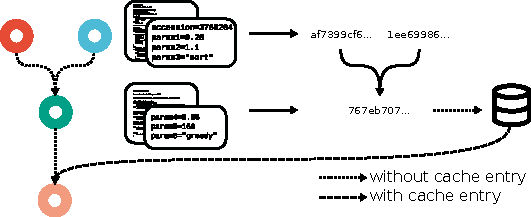
\includegraphics[width=0.7\textwidth]{caching.pdf}
	\caption{
		Blockchain based between workflow caching scheme of Snakemake.
		If a job is eligible for caching, its code, parameters, raw input files, software environment and the hashes of its dependencies are used to calculate a SHA-256 hash value, under which the output files are stored in a central cache.
		Subsequent runs of the same job (with the same dependencies) in other workflows can skip the execution and directly take the output files from the cache.
	}
	\label{fig:caching}
\end{figure}

The hash value is calculated in the following way.
Let $J$ be the set of jobs of a workflow.
For any job $j \in J$, let $c_j$ denote its code (shell command, script, wrapper, or notebook), let $P_j = \{(k_i, v_i) \mid i=0,\dots,m\}$ be its set of parameters (with key $k_i$ and JSON-encoded value $v_i$), let $F_j$ be its set of input files that are not created by any other job, and let $s_j$ be a string describing the associated software environment (either a container URL, a conda environment definition, or both).
Then, assuming that job $j \in J$ with dependencies $D_j \subset J$ is the job of interest, we can calculate the hash value as $$ h(j) = h'\left( c_j \oplus \left(\bigoplus_{i=0}^m k_i \oplus v_i \right) \oplus \left( \bigoplus_{f \in F_j} h'(f) \right) \oplus s_j \oplus \left( \bigoplus_{j' \in D_j} h(j') \right) \right) $$ with $h'$ being the SHA256 \parencite{Handschuh} hash function, $\oplus$ being the string concatenation, and $\bigoplus$ being the string concatenation of its operands in lexicographic order.

The hash function $h(j)$ hence comprehensively describes everything that affects the content of the output files of job~\(j\), namely code, parameters, raw input files, software environment and input generated by jobs it depends on.
For the latter, we recursively apply the hash function~\(h\) again.
In other words, for each dependency~\(j' \in D_j\) we include a hash value into the hash of job~\(j\), which is in fact the hashing principle behind blockchains \parencite{narayanan_bitcoin_2016}.

\subsubsection{Graph partitioning}\label{sec:partitioning}

A data analysis workflow can consist of a diversity of different computing jobs, some of which will be long running, and some might be very short running (down to a few seconds or even less).
When executing a Snakemake workflow in a cluster or cloud setting, by default every job will be submitted separately to the underlying queuing system.
For short running jobs, this can result in a considerable overhead, as they will have to wait in a queue, and also might cause additional delays or costs when accessing files from remote storage or network file systems.
To minimize such overhead, Snakemake offers the ability to partition the DAG of jobs into subgraphs that will be submitted together, as a single cluster or cloud job.

Partitioning happens by assigning rules to groups (see \autoref{fig:grouping}).
Upon execution, Snakemake determines connected subgraphs with the same assigned group for each job, and submits such subgraphs together (as a so called \emph{group job}) instead of submitting each job separately.
For each group, it is in addition possible to define how many connected subgraphs shall be spanned when submitting (one by default).
This way, it is possible to adjust the partition size to the needs of the available computational platform.
The resource usage of a group job is determined by sorting involved jobs topologically, summing resource usage per level and taking the maximum over all levels.

\begin{figure}
	\image{group-jobs.pdf}
	\caption{Job graph partitioning by assigning rules to groups.
		Two rules of the example workflow (\autoref{fig:example}a) are grouped together, (a) spanning one connected component, (b) spanning two connected components, and (c) spanning five connected components.
		Resulting submitted group jobs are represented as grey boxes.
	}\label{fig:grouping}
\end{figure}

\subsubsection{Streaming}\label{sec:streaming}

Sometimes, intermediate results of a data analysis can be huge, but unimportant enough to not store them on disk.
Apart from the option to mark such files as temporary, so that Snakemake automatically deletes them once not needed anymore, it is also possible to instruct Snakemake to never store them on disk at all, but instead directly stream their content from the producing job to to the consuming job.
This implies that the producing and consuming jobs have to run at the same time on the same computing node (then, the output of the producer can be written to a small in-memory buffer; on Unix, this is called a named pipe).
Snakemake ensures this by submitting producer and consumer as a group job (see \autoref{sec:partitioning}).

\section{Conclusion}

While having been almost the holy grail of data analysis workflow management in recent years and being certainly of high importance, reproducibility alone is not enough to sustain the hours of work that scientists invest in crafting data analyses.
Here, we outlined how the interplay of automation, scalability, portability, readability, traceability, and documentation can help to reach beyond reproducibility, making data analyses adaptable and transparent.
Adaptable data analyses can not only be repeated on the same data, but also be modified and extended for new questions or scenarios, thereby greatly increasing their value for both the scientific community and the original authors.
While reproducibility is a necessary property for checking the validity of scientific results, it is not sufficient.
Being able to reproduce exactly the same figure on a different machine tells us that the analysis is robust and valid from a technical perspective.
However, it does not tell anything about the methodological validity (correctness of statistical assumptions, avoidance of overfitting, etc.)
.
The latter can only be secured by having a transparent yet accessible view on the analysis code.

By analyzing its readability and presenting its modularization, portability, reporting, scheduling, caching, partitioning, and streaming abilities, we have shown how Snakemake supports all these aspects, and thereby provides a comprehensive framework for sustainable data analysis.

\section{Author contributions}
Felix Mölder has designed and implemented the job scheduling mechanism (\autoref{sec:scheduling}).
Kim Philip Jablonski has designed and implemented Jupyter notebook integration (\autoref{sec:modularization}).
Michael Hall and Brice Letcher have designed and implemented automated code formatting (\autoref{sec:style}).
Vanessa Sochat has designed and implemented the Google Life Science API execution backend, as well as various improvements to Google storage support (\autoref{sec:scalability}).
Soo Lee has designed and implemented the AWS execution backend via integration with Tibanna (\autoref{sec:scalability}).
Sven O.
Twardziok and Alexander Kanitz have designed and implemented the TES execution backend (\autoref{sec:scalability}).
Manuel Holtgrewe has designed and implemented benchmarking support (supplementary \autoref{s-sec:design-patterns}).
Jan Forster has designed and implemented meta-wrapper support (\autoref{sec:modularization}).
Chris Tomkins-Tinch has designed and implemented remote storage support (\autoref{sec:automation}).
Christian Meesters has supervised the implementation of an initial prototype of the graph partitioning functionality (\autoref{sec:partitioning}).
Sven Nahnsen has provided the initial idea of using blockchain hashing to fingerprint output files a priori.
Johannes Köster has written the manuscript and implemented all other features that occur in the text but are not explicitly mentioned in above listing.

\section{Acknowledgements}
We deeply thank all contributors to the Snakemake, Snakemake-Profile, Snakemake-Workflows, and Snakemake-Wrappers codebase.

\printbibliography
\end{document}
